\section{İndeks Teorisi}

\begin{justify}
Faz düzleminde kapalı eğriler yalnızca yörüngeleri değil, aynı zamanda bu eğrilerin içinde kalan sabit noktalar hakkında da bilgi taşır. İndeks teorisi bu fikri nicelleştirir. Amaç, bir kapalı eğri boyunca vektör alanının kaç kez döndüğünü sayarak eğrinin içinde hangi tür sabit noktaların bulunabileceğini anlamaktır.

Önce sabit nokta içermeyen, basit kapalı bir eğri $C$ seçelim. Eğri üzerinde saat yönünün tersine bir tur atarken vektör alanı $\mathbf{f}(x,y)=(\dot{x},\dot{y})$ her noktada sıfırdan farklı bir vektör verir. Bu vektörün yatay eksenle yaptığı açı $\phi$ olsun. Eğri boyunca bir tam tur sonunda $\phi$ açısının toplam değişimi $2\pi$'nin tam katı olmak zorundadır. Bu tam sayıya $C$ eğrisinin indeksi denir:
\begin{equation}
I_C=\frac{1}{2\pi}\Delta\phi.
\end{equation}

Başka bir deyişle indeks, vektör alanı oklarının eğri boyunca kaç tam dönüş yaptığını ölçer. Eğer oklar toplamda bir kez saat yönünün tersine dönerse $I_C=1$, bir kez saat yönünde dönerse $I_C=-1$ olur. Hiç net dönüş yoksa indeks sıfırdır.

\begin{figure}[H]
\centering
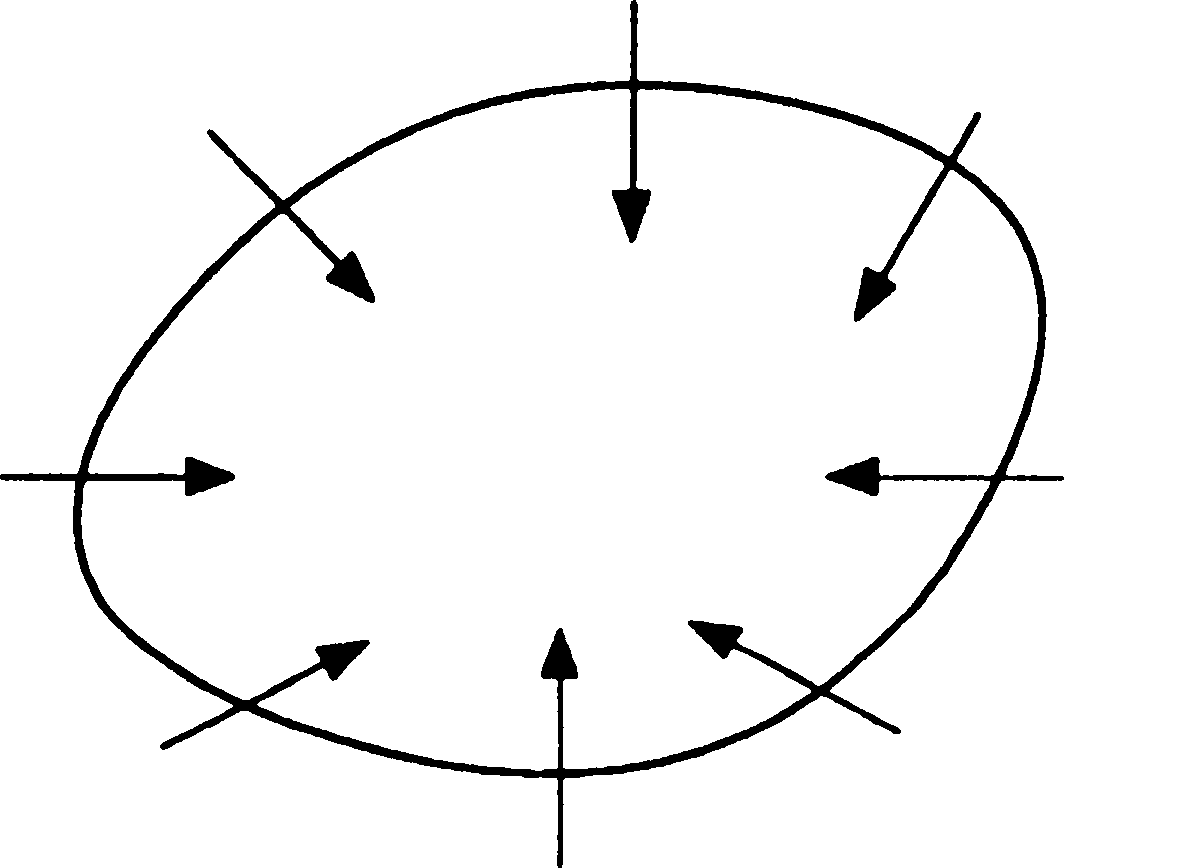
\includegraphics[width=0.82\textwidth]{images/Figures/figur-035.png}
\caption{Kapalı bir eğri boyunca vektör alanı yönünün dönmesi ve indeksin tanımı.}
\label{fig:6-8-1}
\end{figure}

İndeksin en önemli özelliği topolojik kararlılığıdır. Eğri, üzerinden sabit nokta geçirmeyecek biçimde sürekli olarak deforme edilirse indeks değişmez. Çünkü vektör alanı eğri üzerinde hiçbir zaman sıfır olmadığı sürece $\phi$ açısındaki toplam dönüş ancak sürekli değişebilir; fakat indeks bir tam sayı olduğundan sıçrama yapmadan değişemez.
\end{justify}

\subsection*{Sabit Noktaların İndeksi}
\addcontentsline{toc}{subsection}{Sabit Noktaların İndeksi}

\begin{justify}
Yalıtılmış bir sabit noktanın indeksi, bu noktayı çevreleyen küçük bir kapalı eğrinin indeksi olarak tanımlanır. Eğri yeterince küçük seçildiğinde başka sabit nokta içermez; bu nedenle elde edilen sayı yalnızca sabit noktanın yerel yapısına bağlıdır.

Düğüm, spiral ve merkez tipindeki sabit noktaların indeksi $+1$'dir. Bu durum sezgisel olarak açıktır: Bu noktaların çevresinde dolaşırken vektör alanı da bir tam tur döner. Buna karşılık eyer noktasının indeksi $-1$'dir. Eyerin kararlı ve kararsız doğrultuları vektör alanının yönünü öyle değiştirir ki toplam dönüş saat yönünde bir tur olur.

\begin{figure}[H]
\centering
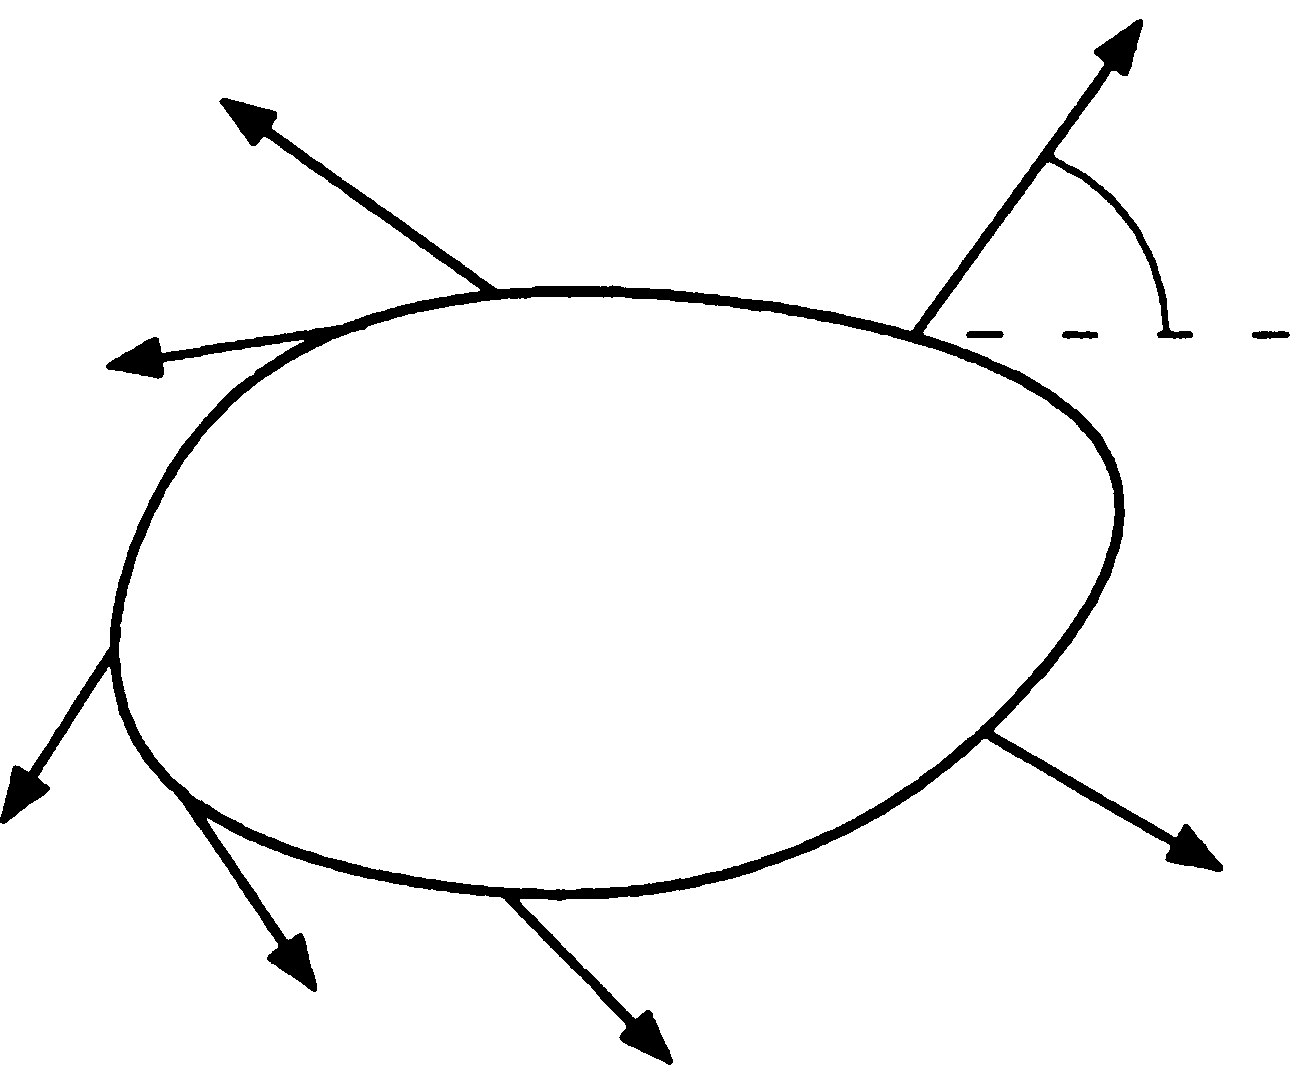
\includegraphics[width=0.82\textwidth]{images/Figures/figur-036.png}
\caption{Düğüm, spiral, merkez ve eyer noktalarının indeksleri.}
\label{fig:6-8-2}
\end{figure}

Bu sonuçlar doğrusal sistemler üzerinden de görülebilir. Lineerleştirme matrisi tekil değilse, sabit nokta hiperboliktir ve yerel faz portresi doğrusal sistemle aynı topolojik tipe sahiptir. Bu durumda
\begin{equation}
\text{indeks}=\operatorname{sgn}(\det A)
\end{equation}
şeklinde yorumlanabilir. $\det A>0$ olduğunda düğüm, spiral ya da merkez benzeri davranış ortaya çıkar ve indeks $+1$ olur. $\det A<0$ olduğunda sabit nokta eyer noktasıdır ve indeks $-1$ olur.
\end{justify}

\subsection*{İndekslerin Toplanması}
\addcontentsline{toc}{subsection}{İndekslerin Toplanması}

\begin{justify}
Bir kapalı eğri $C$ içinde sonlu sayıda yalıtılmış sabit nokta bulunsun ve eğrinin üzerinde sabit nokta olmasın. Bu durumda $C$ eğrisinin indeksi, içerdiği sabit noktaların indekslerinin toplamına eşittir:
\begin{equation}
I_C=\sum_{k} I_k.
\end{equation}

Bu kural faz portrelerini hızlı biçimde denetlemek için çok yararlıdır. Örneğin kapalı bir eğrinin indeksi $+1$ ise, eğrinin içinde yalnızca bir merkez bulunabilir; ya da bir eyer ve iki düğüm gibi toplam indeksi yine $+1$ yapan başka kombinasyonlar olabilir. Fakat tek başına bir eyer, indeksi $-1$ olduğundan böyle bir eğrinin içinde bulunamaz.

\begin{figure}[H]
\centering
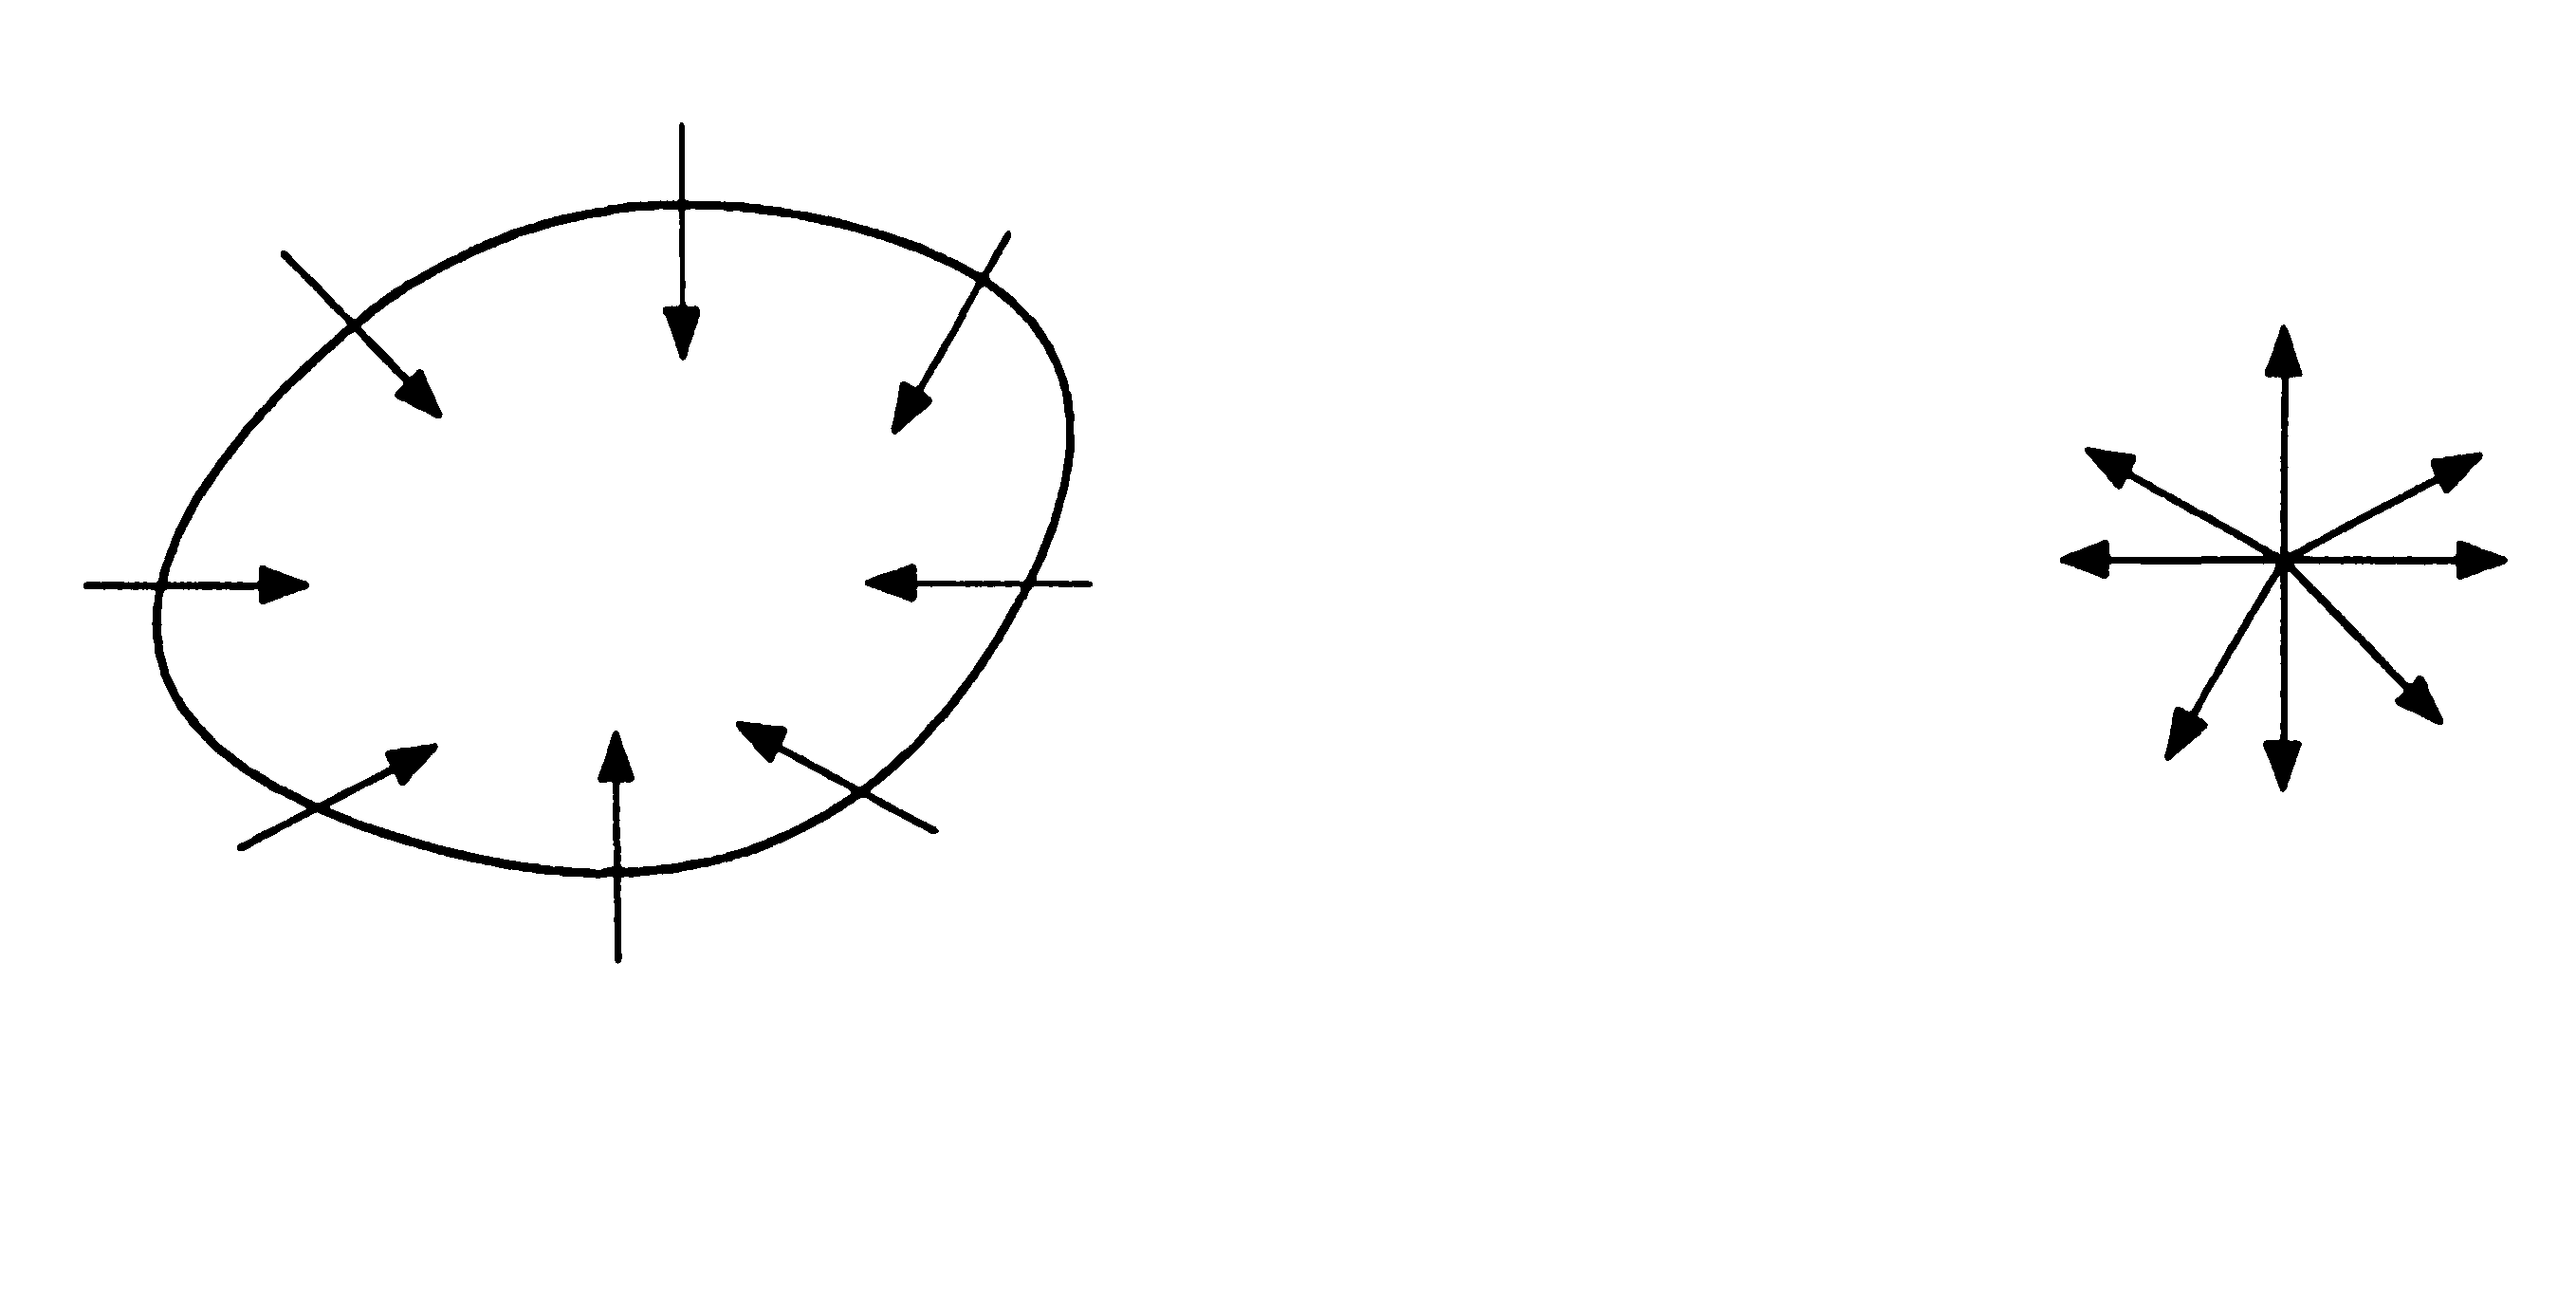
\includegraphics[width=0.82\textwidth]{images/Figures/figur-037.png}
\caption{Bir kapalı eğrinin indeksinin içerdiği sabit noktaların indeksleri toplamına eşit olması.}
\label{fig:6-8-3}
\end{figure}

Özel olarak, kapalı bir yörüngeyi ele alalım. Yörüngenin kendisi boyunca vektör alanı eğriye teğettir ve hareket yönünü gösterir. Kapalı yörünge bir tur tamamladığında teğet vektörü de bir tam tur döner. Dolayısıyla kapalı yörüngenin indeksi
\begin{equation}
I_C=1
\end{equation}
olur. Buradan önemli bir sonuç çıkar: Her kapalı yörüngenin içinde toplam indeksi $+1$ olan en az bir sabit nokta bulunmalıdır.

\begin{figure}[H]
\centering
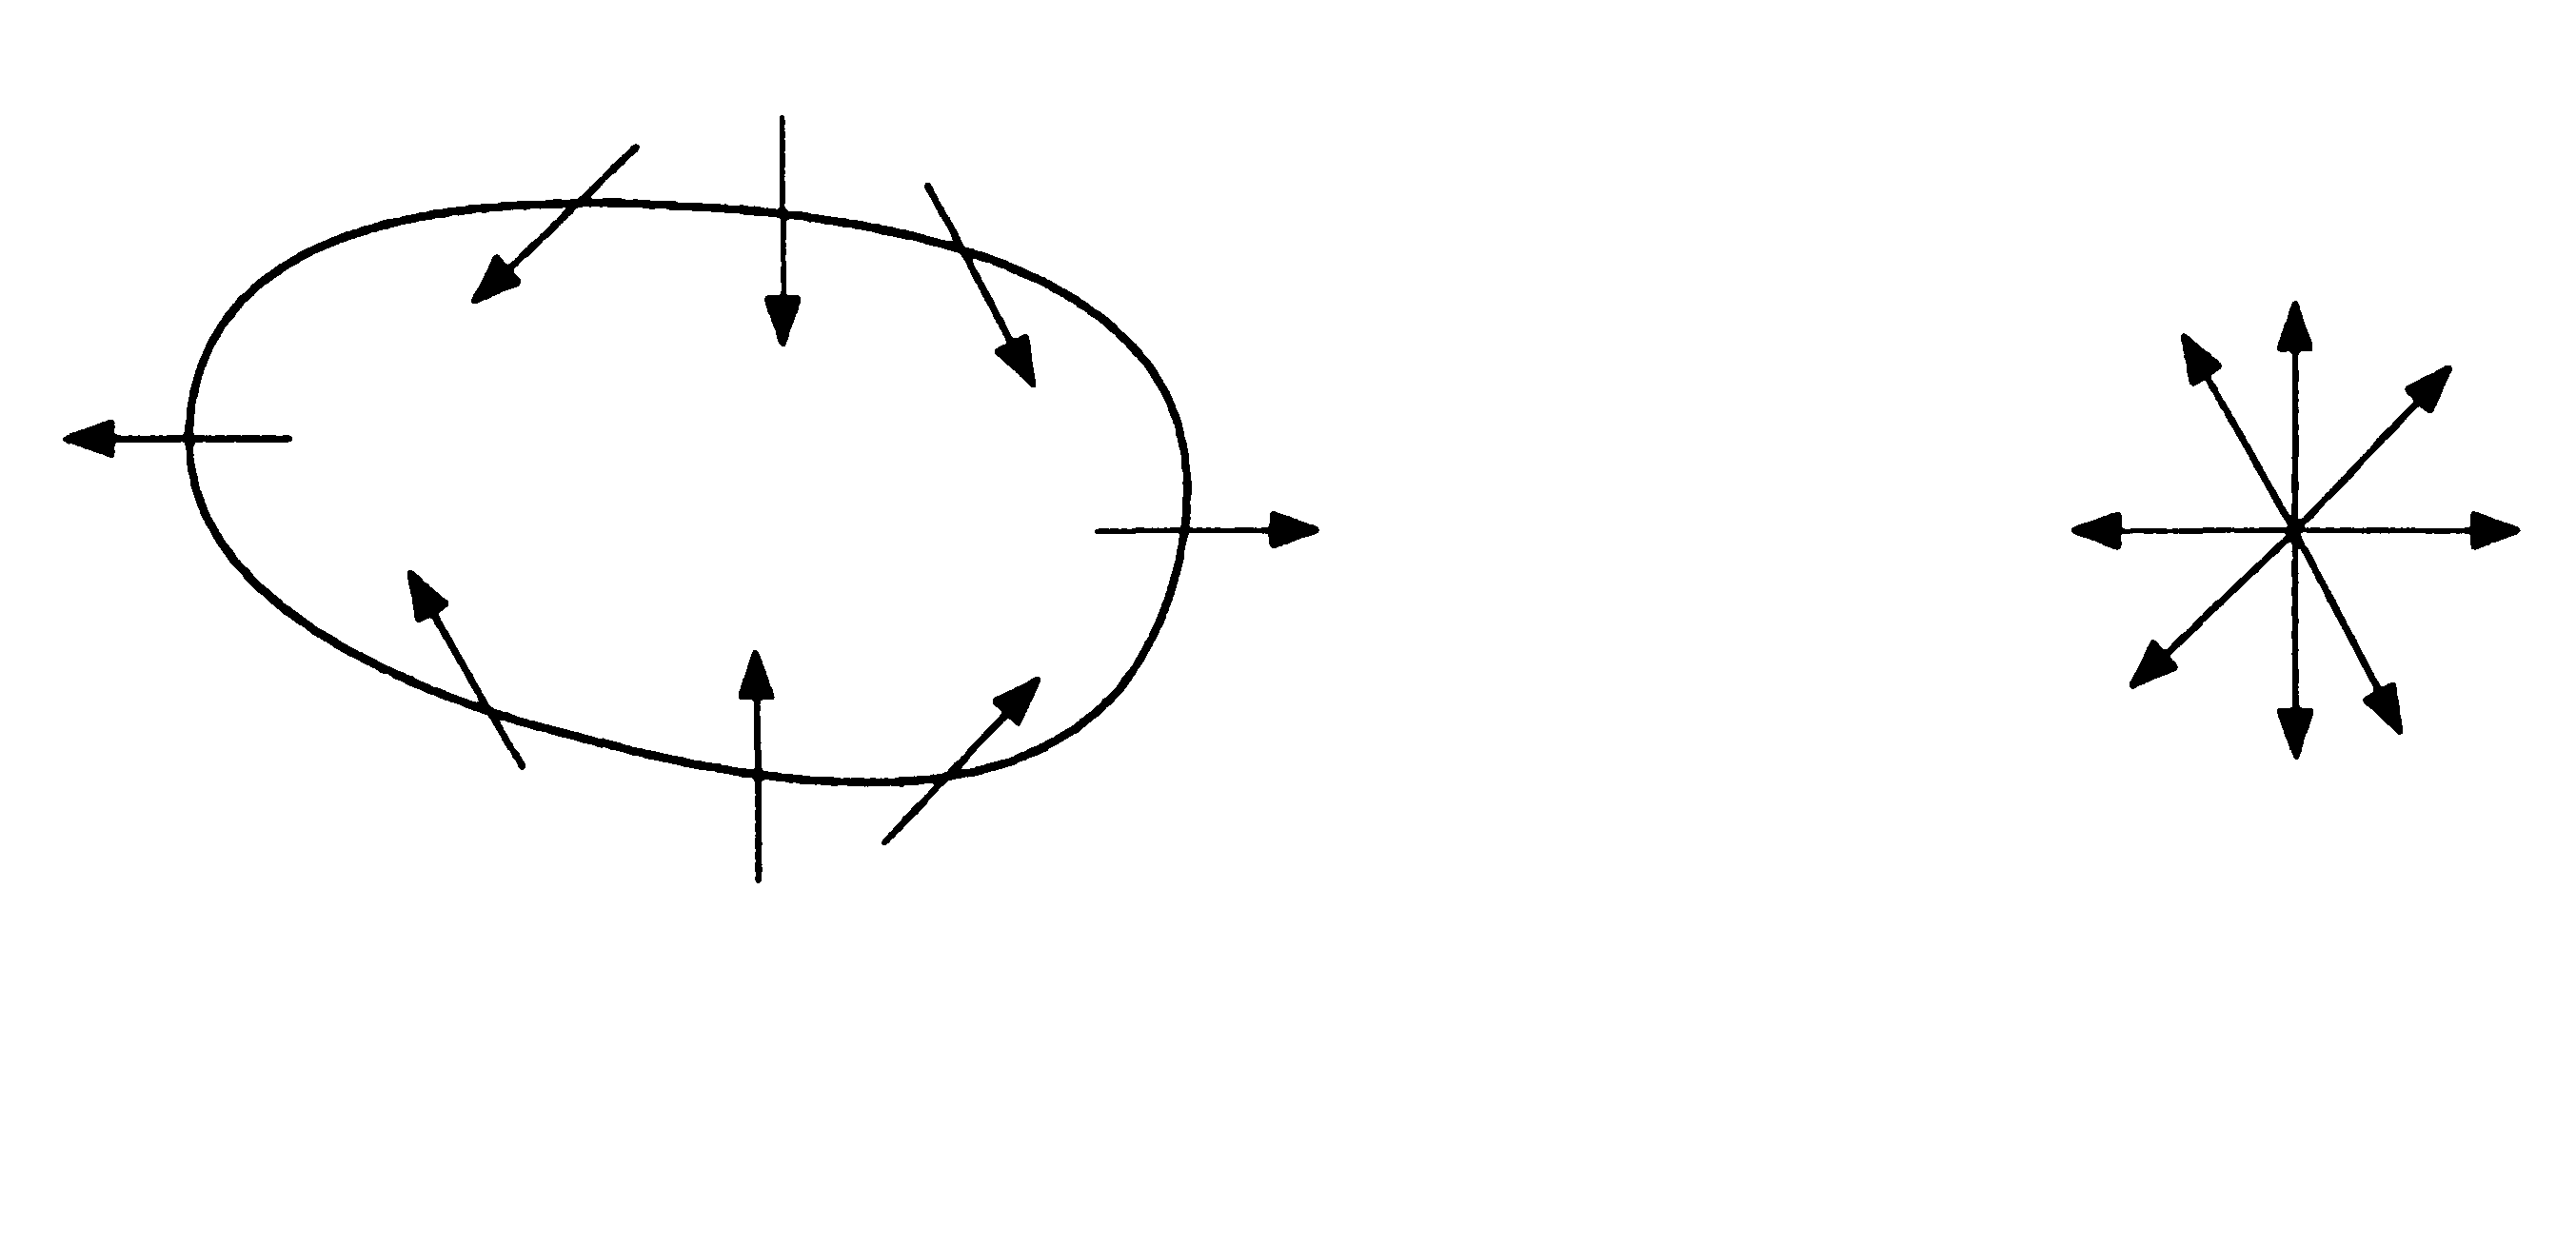
\includegraphics[width=0.82\textwidth]{images/Figures/figur-038.png}
\caption{Kapalı bir yörüngenin indeksinin $+1$ olması.}
\label{fig:6-8-4}
\end{figure}
\end{justify}

\subsection*{Örnek 6.8.1}
\addcontentsline{toc}{subsection}{Örnek 6.8.1}

\begin{justify}
Bir faz portresinde kapalı bir yörüngenin içinde yalnızca bir sabit nokta bulunduğu gözlensin. Bu sabit nokta eyer olabilir mi?

\textbf{Çözüm.} Hayır. Kapalı yörüngenin indeksi $+1$'dir. Eğer içindeki tek sabit nokta eyer olsaydı, bu noktanın indeksi $-1$ olurdu. İndekslerin toplanması kuralı $+1=-1$ gibi olanaksız bir sonuç vereceğinden, kapalı yörüngenin içinde tek başına eyer noktası bulunamaz. Tek sabit nokta varsa bu noktanın indeksi $+1$ olmalıdır; örneğin merkez, spiral ya da düğüm olabilir.

\begin{figure}[H]
\centering
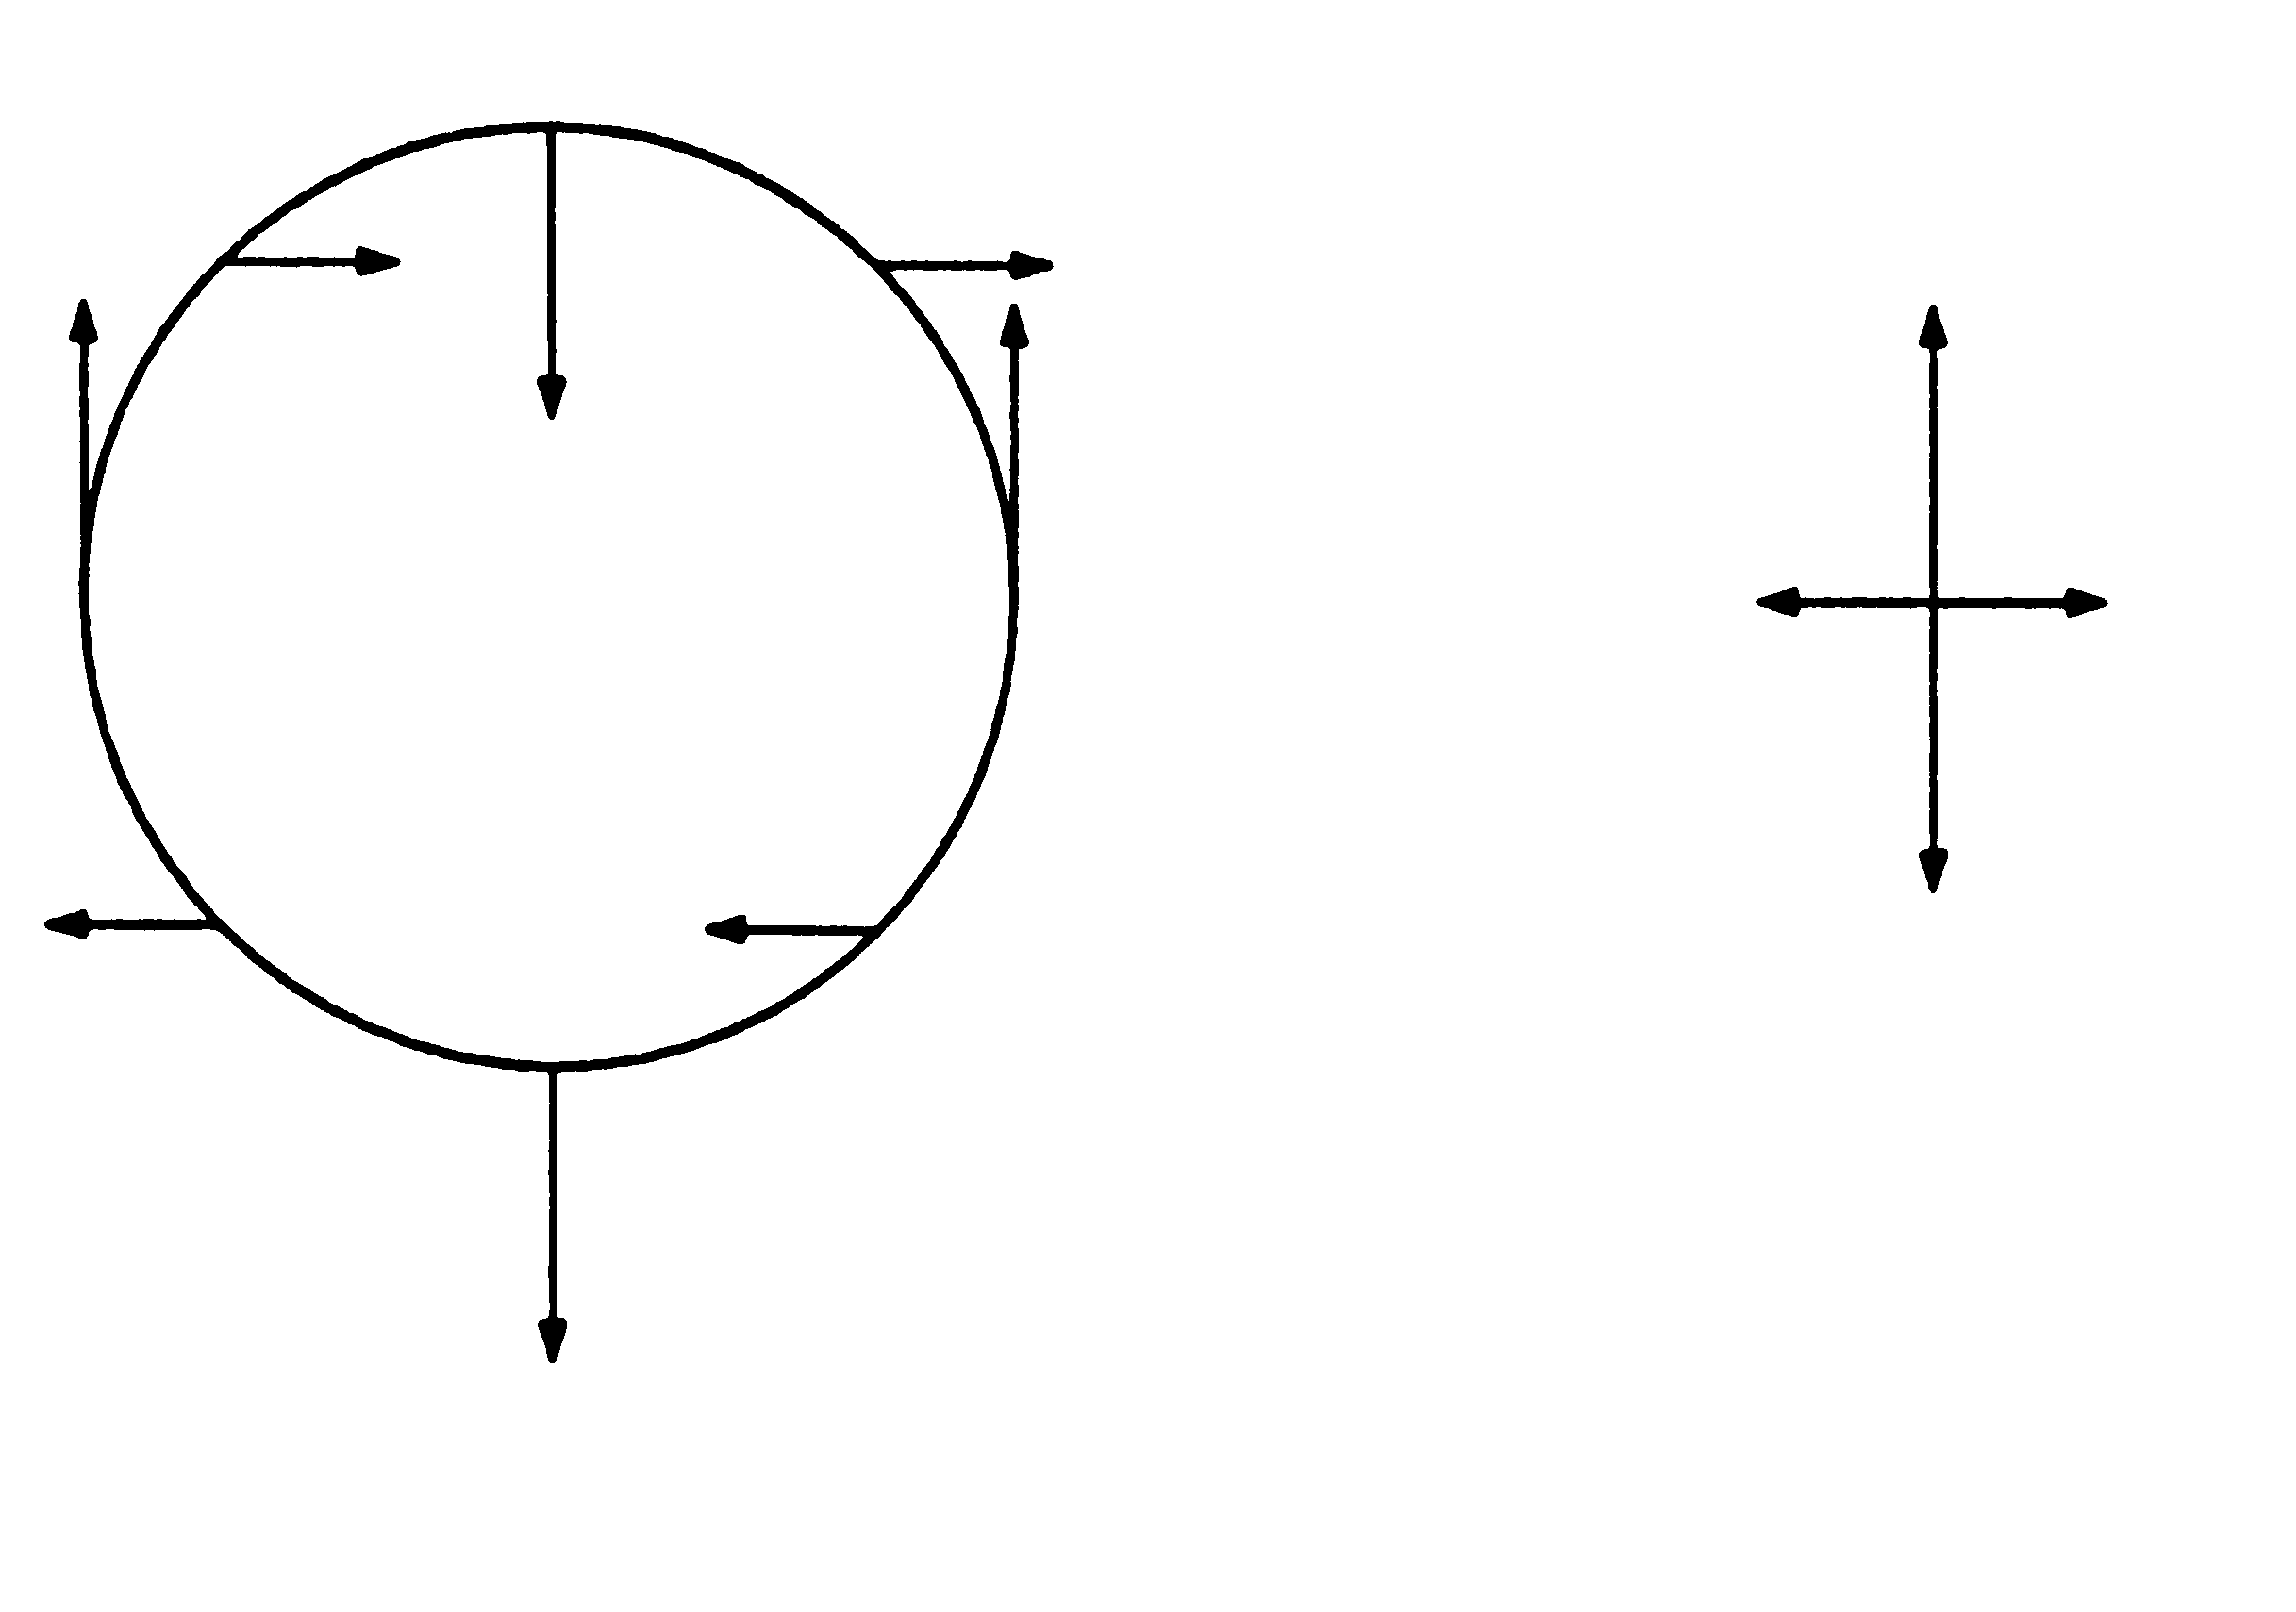
\includegraphics[width=0.82\textwidth]{images/Figures/figur-039.png}
\caption{Kapalı yörüngenin içinde tek başına eyer bulunamaması.}
\label{fig:6-8-5}
\end{figure}
\end{justify}

\subsection*{Örnek 6.8.2}
\addcontentsline{toc}{subsection}{Örnek 6.8.2}

\begin{justify}
Bir kapalı yörüngenin içinde iki eyer noktası varsa, içeride en az kaç tane eyer olmayan sabit nokta bulunmalıdır?

\textbf{Çözüm.} Kapalı yörüngenin indeksi $+1$'dir. İki eyerin toplam indeksi $-2$ olur. Eyer olmayan tipik hiperbolik sabit noktaların her biri $+1$ indeks taşır. Toplamın $+1$ olması için
\begin{equation}
-2+n=1
\end{equation}
olmalıdır. Buradan $n=3$ bulunur. Dolayısıyla içeride en az üç tane eyer olmayan sabit nokta bulunmalıdır.

\begin{figure}[H]
\centering
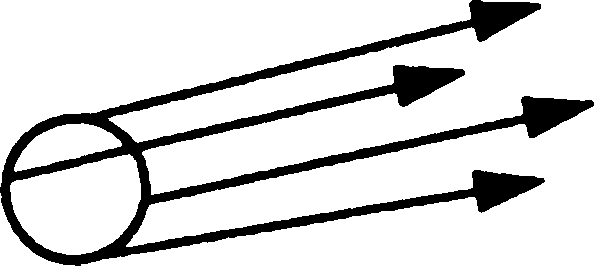
\includegraphics[width=0.82\textwidth]{images/Figures/figur-040.png}
\caption{İki eyer içeren kapalı yörüngede indeks dengesinin sağlanması.}
\label{fig:6-8-6}
\end{figure}
\end{justify}

\subsection*{Sınırlar ve Kullanım}
\addcontentsline{toc}{subsection}{Sınırlar ve Kullanım}

\begin{justify}
İndeks teorisi, faz portrelerinin mümkün olup olmadığını sınamak için güçlü ama kaba bir araçtır. İndeks yalnızca toplam topolojik bilgiyi verir; sabit noktaların tam konumlarını, yörüngelerin biçimini ya da kararlılık şiddetini belirlemez. Buna rağmen yanlış çizilmiş faz portrelerini yakalamakta çok etkilidir.

Örneğin bir kapalı yörüngenin içinde hiçbir sabit nokta çizilmemişse faz portresi eksiktir. Benzer biçimde, kapalı yörünge içinde yalnızca iki eyer noktası çizilmişse toplam indeks $-2$ olur ve bu da kapalı yörüngenin indeksi olan $+1$ ile çelişir. Bu tür denetimler özellikle karmaşık doğrusal olmayan sistemlerde faz portresinin tutarlılığını kontrol etmek için kullanılır.

\begin{figure}[H]
\centering
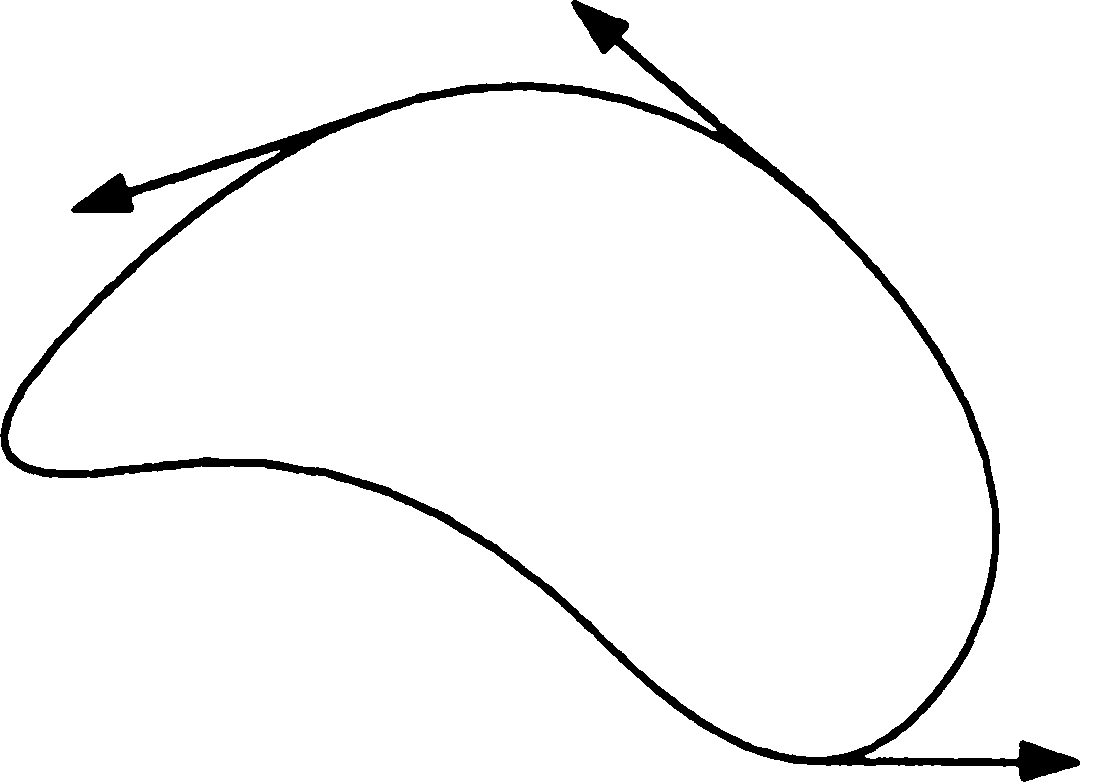
\includegraphics[width=0.82\textwidth]{images/Figures/figur-041.png}
\caption{İndeks kuralıyla elenen tutarsız faz portresi örnekleri.}
\label{fig:6-8-7}
\end{figure}

Sonuç olarak indeks teorisi, yerel sabit nokta analizini küresel faz portresi bilgisiyle birleştirir. Düğüm, spiral, merkez ve eyer gibi yerel yapıların kapalı eğriler içinde nasıl dengelenmesi gerektiğini gösterir.

\begin{figure}[H]
\centering
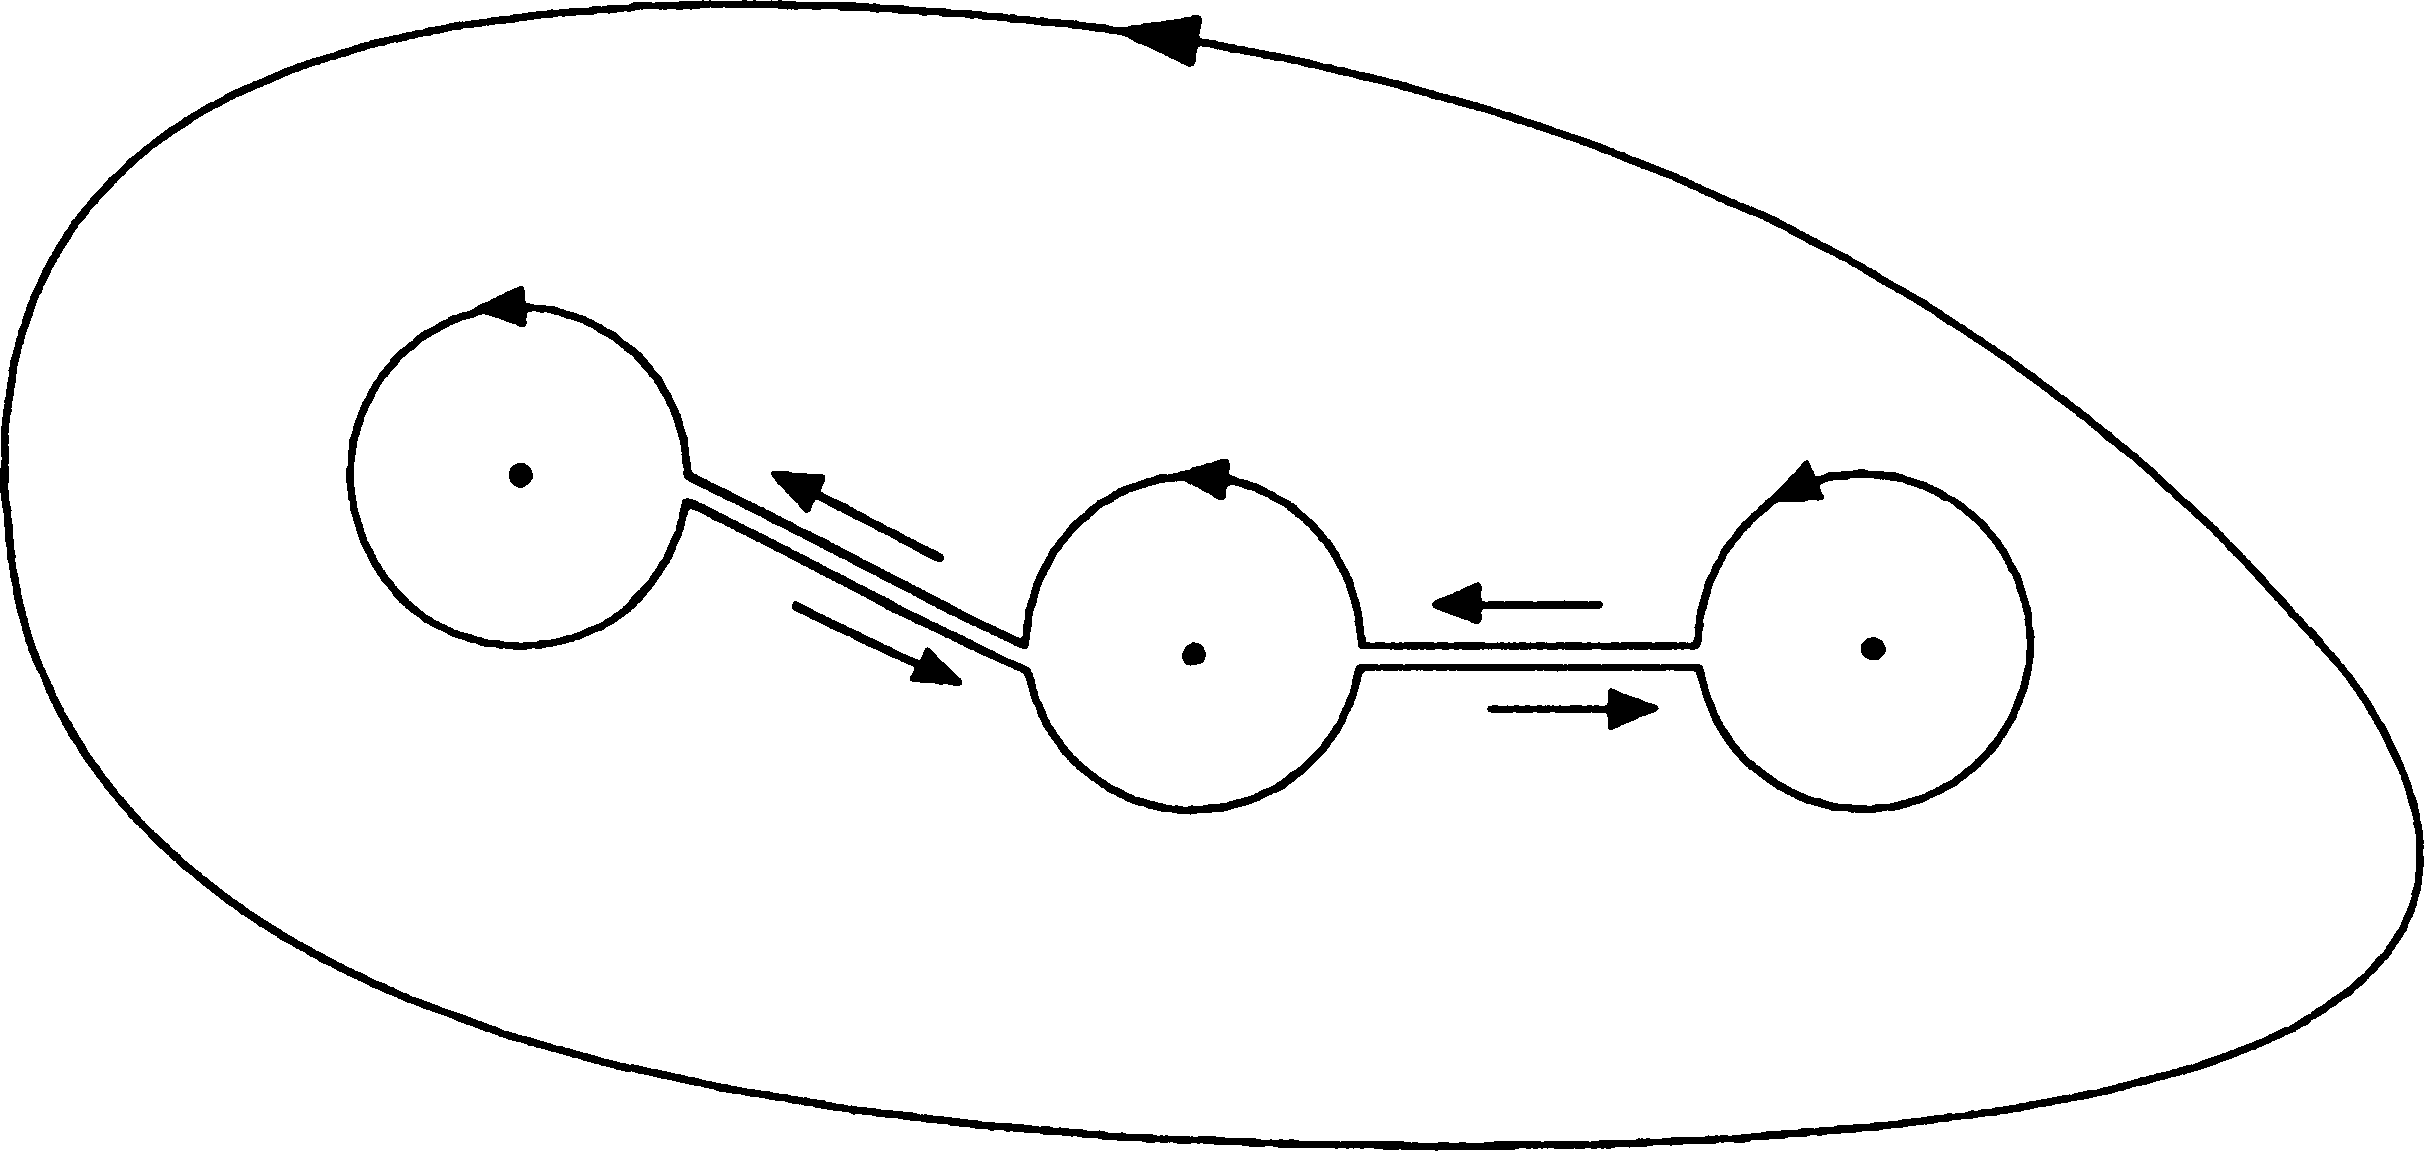
\includegraphics[width=0.82\textwidth]{images/Figures/figur-042.png}
\caption{Yerel sabit nokta indekslerinin küresel faz portresiyle uyumu.}
\label{fig:6-8-8}
\end{figure}
\begin{figure}[H]
\centering
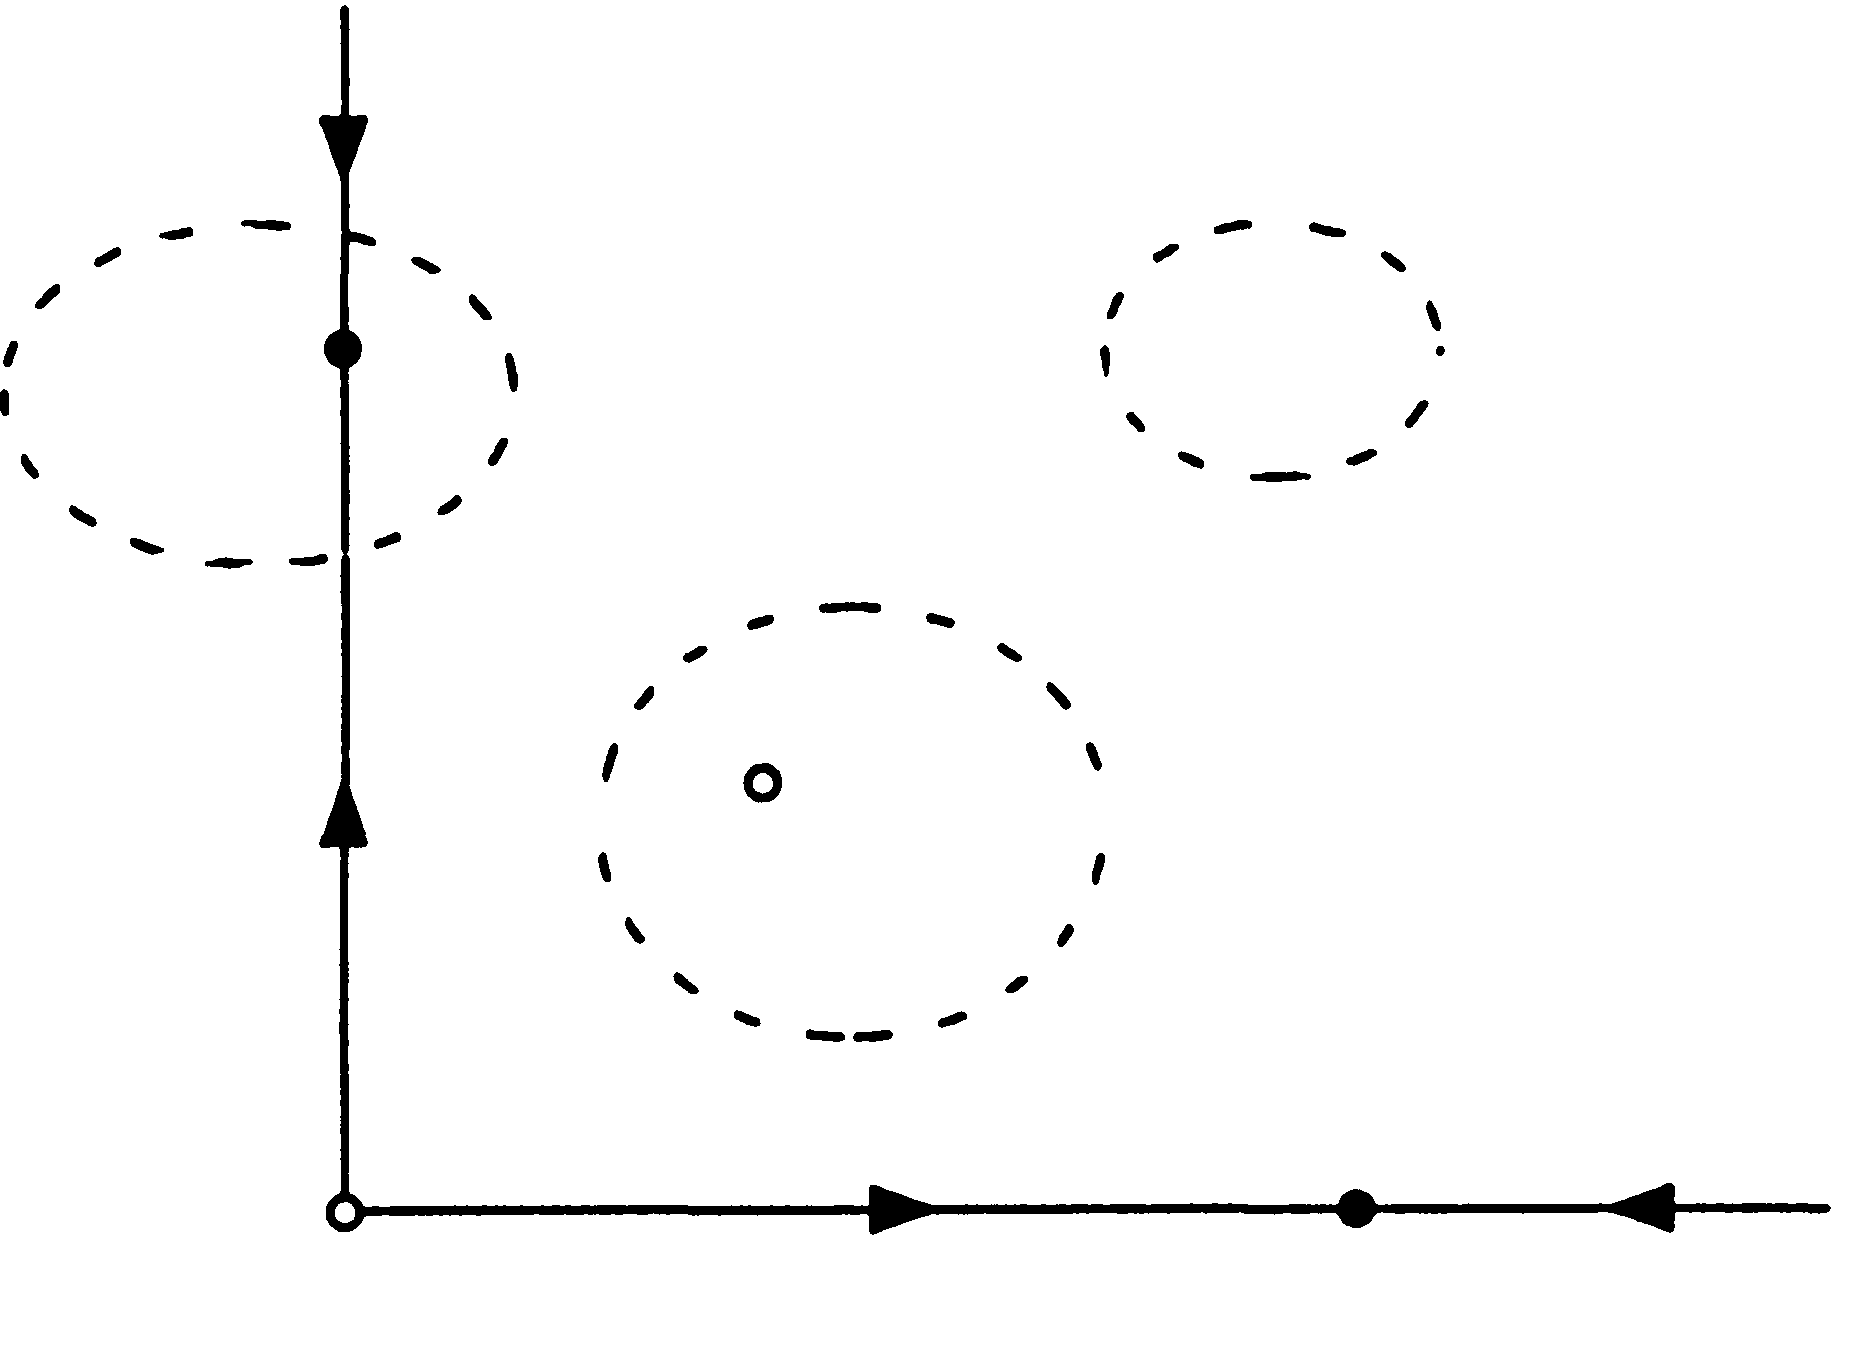
\includegraphics[width=0.82\textwidth]{images/Figures/figur-043.png}
\caption{İndeks teorisiyle faz portresi tutarlılığının özet gösterimi.}
\label{fig:6-8-9}
\end{figure}
\end{justify}